 \section{图与网络规划}
 图与网络规划 (graphics and network programming) 是近几十年来运筹学领域中发展迅速、而且十分灵活的一个分支。由于它对实际问题的描述,具有直观性,
 故广泛应用于物理学、化学、信息论、控制论、计算机科学、社会科学、以及现代经济管理科学等许多科学领域。图与
 网络分析的内容十分丰富,这里只介绍路径规划、网络流、最小生成树、旅行商等几个经典问题。



\subsection{\pkg{igraph} 包在图与网络分析中的应用}
\pkg{igraph} 包\citep{igraph06}是一个非常强大的包,它可以快速轻松地创建、绘制和分析
无向图及有向图 (图的顶点和边允许百万以上!)
,并解决了经典图论问题,如最小生成树、最大网络流量、最短路等问题。该包内容很丰富,下面仅讨论几个常见问题。


\pkg{igraph}包中,\fun{graph.maxflow()} 函数可以解决最大流问题,用法为:

\begin{verbatim}
graph.maxflow(graph, source, target, capacity=NULL)
\end{verbatim}

其中,\rcode{graph} 为要处理的图,为 igraph 格式,其创立方式非常简单,参见帮助文档。
\rcode{source} 和 \rcode{target} 分别代表网络中要求最大流的起始点和终点,\rcode{capacity} 为边的权重。


\fun{minimum.spanning.tree()} 函数可以解决最小生成树问题,用法为:

\begin{verbatim}
minimum.spanning.tree(graph, weights=NULL, algorithm=NULL, ...)
\end{verbatim}

其中,\rcode{graph} 意义同上,\rcode{weights} 为边的权,\rcode{algorithm} 为所选择的算法,如果置空 (默认),
函数将自动选取算法。


\fun{shortest.paths()} 函数可以解决任意两顶点间 (要求边的权非负) 的最短路问题,用法为:

\begin{verbatim}
shortest.paths(graph,v=V(graph),mode=c("all","out","in"),weights=NULL)
\end{verbatim}

其中,\rcode{graph}、\rcode{weight} 意义同上,
\rcode{v} 为该图的顶点 (\verb|V(graph)| 即为求图的顶点),
\rcode{mode} 为字符变量,
当其为 \verb|"all"| 时,忽略图形边的方向,即将图作为无向图 (默认) 来计算最短路程;当其为 \verb|"out"| 时,考虑各个边的方向;
当其为 \verb|"in"| 时,考虑各个边的方向,但此时将各边的方向倒置。因此,\rcode{mode} 取 \verb|"all"| 时,所得的
最短路矩阵为对称的,取 \verb|"out"| 和 \verb|"in"| 时,所得的两个矩阵互为转置矩阵。
\begin{exmp}\label{ex:graph}
图 \ref{fig:graph} 是个有向图\footnote{该图主体是由后面的代码画的。},方向如图中箭头所示,边上的数字为其权重,试求下列问题:\\
 1. 从顶点 0 到顶点 7 的最大流量 (此时图中各条边上的数字代表容量限制);\\
 2. 该连通图的最小生成树;\\
 3. 该图中任意两顶点之间的最短路程 (考虑方向)。
\end{exmp}
\begin{figure}[h]
\centering
\includegraphics[width=8cm]{./pic/graph}
\caption{网络图}\label{fig:graph}
\end{figure}

\noindent{{\textbf  解:}这三个问题是图论中的典型问题。首先,应该在 \R 中构造该图,然后分别调用相关命令即可。
\R 代码及运行结果如下:}
\begin{Verbatim}
> library(igraph)                               #载入包
> e = matrix(nc = 3, byrow = TRUE, c(0,1,5, 0,2,4, 0,3,3, 1,5,3, 1,4,5,
+         2,5,3, 2,6,2, 3,6,2, 4,1,5, 4,7,4, 5,7,3, 6,7,5)) #边的权矩阵
> g = add.edges(graph.empty(8), t(e[,1:2]), weight = e[,3]) #构造图
> tkplot(g)                                     #绘制网络图
[1] 35
> graph.maxflow(g, 0,7, capacity = E(g)$weight) #最大流
[1] 11
> mst = minimum.spanning.tree(g)                #最小生成树
> tkplot(mst)                                   #绘制最小生成树
[1] 36
> (tree_min = sum(E(mst)$weight))               #计算并输出最小生成树的权
[1] 20
> shortest.paths(g, mode = "out")               #最短路矩阵
     [,1] [,2] [,3] [,4] [,5] [,6] [,7] [,8]
[1,]    0    5    4    3   10    7    5   10
[2,]  Inf    0  Inf  Inf    5    3  Inf    6
[3,]  Inf  Inf    0  Inf  Inf    3    2    6
[4,]  Inf  Inf  Inf    0  Inf  Inf    2    7
[5,]  Inf    5  Inf  Inf    0    8  Inf    4
[6,]  Inf  Inf  Inf  Inf  Inf    0  Inf    3
[7,]  Inf  Inf  Inf  Inf  Inf  Inf    0    5
[8,]  Inf  Inf  Inf  Inf  Inf  Inf  Inf    0
\end{Verbatim}
\begin{figure}[h]
\centering
\includegraphics[width=8cm]{./pic/tree.pdf}
\caption{最小生成树图}\label{fig:tree}
\end{figure}

图 \ref{fig:graph} 为所画的网络图 (边上的数字由其它软件所绘)。图 \ref{fig:tree} 为最小生成树图。


由第 8 行可知,最大流为 11。由第 13 行可知,最小生成树的权为 20。由 15 -- 23 行 (最短路矩阵) 可以知道该网络上每
两个定点的最短路。如顶点 0 到顶点 7 的最短路为 10(矩阵中第 1 行第 8 列对应的元素)。需要说明的是,第 6,11 行结果
表示这是 \R 软件打开的第 35,36 个 tk 图形设备,与本题的具体内容无关。


观察以上代码和输出结果,发现 \R 仅仅用短短十行代码,就解决了最大流问题、最短路问题、最小生成树问题,并绘制出两个相关的
图形,其效率之高,令人叹为观止。而 LINGO 则需要针对每个问题输入不同模型、约束条件等,远远不如 \R 效率高,
至于绘图功能,LINGO 还需要很大的改进。
\subsection{专题:旅行商问题}
 旅行商问题即 TSP 问题 (travelling salesman problem):假设有一个人要游览 n 个城市,并且每个城市只能去一次,
 而且最后要回到原点,问他应该选取什么路线才能是总路线最短。旅行商问题易于描述但难于解决,是著名的 NP 难题之一 (有
  n 个城市时,路线组合数为 $(n-1)!/2$,组合数呈爆炸式增长),
 至今世界上还有不少人在研究它。解决该问题的算法也层出不穷,如动态规划、模拟退火算法、遗传算法、禁忌算法、蚁群算法等等。
 
 
 TSP 问题可分为对称型和非对称型两种,对称型即两地之间的距离没有方向性,即 a 地到 b 地的距离恒
 等于 b 地到 a 地的距离,而非对称问题中,则没有这个限制。\R 中,有专门解决 TSP 问题的包 \pkg{TSP} \citep{TSP08}。
 常用函数有 \fun{TSP()},\fun{ATSP()},\fun{solve\_TSP()},\fun{tour\_length()} 等。
 其中 \fun{TSP()} 和 \fun{ATSP()} 函数分别将对称矩阵、一般矩阵
处理为函数 \fun{solve\_TSP()} 所需要的数据格式。
\fun{solve\_TSP()} 为核心的求解函数,其用法为:

\begin{verbatim}
solve_TSP(x, method, control)
\end{verbatim}

其中,前两个参数比较常用,\rcode{x} 为 TSP 或 ATSP 格式,\rcode{method} 为所用的算法,选项有
 \rcode{nearest\_insertion}, \rcode{farthest\_insertion},
\rcode{arbitrary\_insertion},  \rcode{2-opt}, \rcode{nn} 等近十种
启发式算法\footnote{算法原理参见帮助文档。}。
%\rcode{arbitrary\_insertion}、\rcode{nn}、\rcode{repetitive\_nn}、
函数 \fun{tour\_length()} 计算所得路线的总长度。


由于 TSP 问题非常复杂,建议在解决规模较大 TSP 问题的的时候,不妨利用多种算法多次计算得到众多
 解后,再从中选择一个最好的作为最终解。下面结合具体例子来说明该函数的用法。
 \begin{exmp}\label{ex:path_china}
 走遍中国问题:你我周游全国,从北京出发,要遍游我国 34 个省级行政中心,最后要回到北京。假设各城市之间的
 路程可以视为它们在地球球面\footnote{地球为椭圆,但很近似于正圆,在这里将地球视为球体并不影响结果。}上的最短距离,
 请设计一条路线使得总行程最短。
 \end{exmp}

\noindent{{\textbf  解:}这是一个典型的对称 TSP 问题,通过组合数学知识,可知路线组合总数共有 $4.341659*10^{36}$ 种!}


 首先,获得 34 个省级行政中心的经纬度数据,
 根据空间几何知识,计算出它们两两之间的球面距离,然后调用 \pkg{TSP} 包中的相关函数即可得到最短路线。
 最后,还可以利用 \R 中的 \pkg{maps}\citep{maps08}, \pkg{maptools}\citep{maptools08}等包将所得路线以及城市画在中国地图上,
 得到一个直观、漂亮的结果。\R 代码如下:
 \VerbatimInput{./code/tsp.r}
 \begin{figure}[h]
\centering
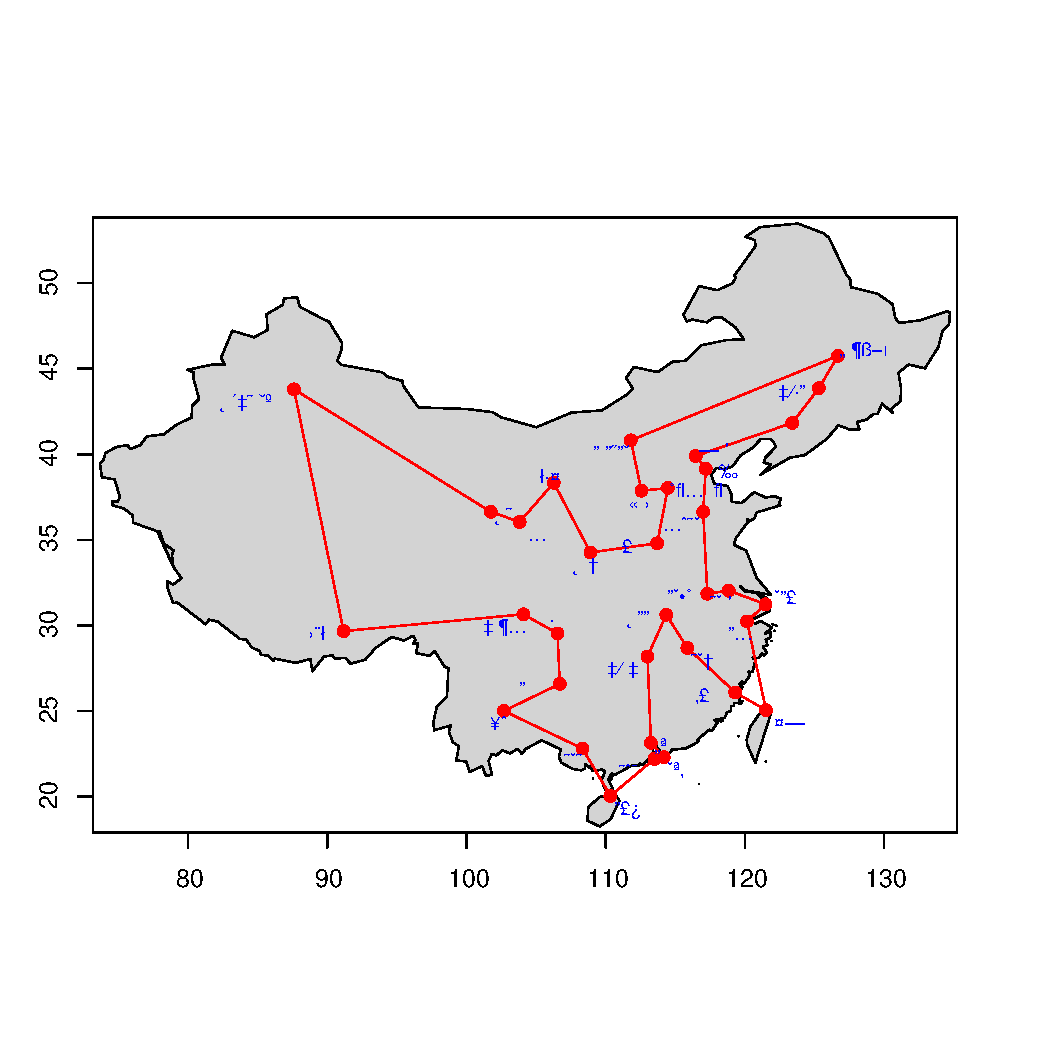
\includegraphics[width=12cm]{./pic/china.pdf}
\caption{走遍中国线路}\label{fig:path_china}
\end{figure}

上面程序中:第 4 行读取的 csv 格式
数据共有 3 列,分别为城市名、经度、纬度。
第 30 行中,\fun{pointLabel()} 函数将城市名标在地图上,
为了使它们重叠最小,该函数可以使用模拟退火算法 (默认) 或遗传算法来优化文本标签的放置位置。


多次运行程序,所得的最短路程\footnote{不能保证是全局最优解。}为 15638.01 千米,路线为
北京    、 天津    、 济南 、合肥    、 南京    、 上海 、杭州    、 台北    、 福州 、
南昌    、 武汉    、 长沙 、广州    、 香港    、 澳门 、海口    、 南宁    、 昆明 、
贵阳    、 重庆    、 成都 、拉萨    、 乌鲁木齐、 西宁 、兰州    、 银川    、 西安 、
郑州    、 石家庄  、 太原 、呼和浩特、 哈尔滨  、 长春 、沈阳    、 北京。
将路线画在中国地图上,如图 \ref{fig:path_china}。


另外,该包还提供了到 Concorde TSP Solver\footnote{需要单独下载,地址为 \url{http://www.tsp.gatech.edu/concorde/index.html}} 的接口,
Concorde TSP Solver 是一个专门解决 TSP 问题的开源软件包,有成功解决 15112 个城市的 TSP 问题的辉煌
战绩\footnote{根据斯特林公式,此时总的路线数约有 $15111!/2\approx4*10^{56593}$ 种。}。


通过此例,可以发现 \R 在读取数据、编程计算、绘图上都非常灵活强大 (熟悉 LINGO 软件的朋友应该更深有体会),
并且由于世界上各个领域内专家的无私贡献,\R 有了各种各样的包,可以便捷地解决各类问题。\R 不仅仅是一个统计软件,
而是一个由奉献者构建起来的平台,在这个平台上,我们可以随心所欲地解决各类问题,也可以将自己的优秀思想加进去。
众人拾柴火焰高,\R 的强大来自于大家。
